\documentclass[12pt]{elsarticle}
\usepackage{newtxtext}
\usepackage[margin=1in]{geometry}
%\pagestyle{empty}
\usepackage{natbib}
\bibliographystyle{abbrvnat}
\usepackage{color}
\usepackage{amsmath}
\usepackage{hyperref}
\usepackage{wrapfig}
\usepackage{titlesec}
\usepackage{colortbl}
\titleformat{\section}[runin]{\normalfont\bfseries}{\thesection.}{3pt}{}


\begin{document}

\begin{center} \textbf{PROJECT NARRATIVE} \end{center}

%
\section{Goals and objectives} 
\subsection{Goals}
\begin{enumerate}
\item To contribute our skills in economics and optimization to maximizing the returns on investment from barrier culvert restoration in Washington State.
\item To learn about the diverse priorities, objectives, and concerns of various stakeholders as relates to barrier culvert restoration in Washington State.
\item To train graduate students in producing high-quality, relevant, and reproducible applied research.
\end{enumerate}

\subsection{Objectives}
\begin{enumerate}
\item Catalog methods and datasets for fish passage prioritization indices for all counties, and any other entities using prioritization indices, within the Washington state injunction area. 
\item Generate consistent predicted cost estimates for all barriers to fish passage within the Washington state injunction area. 
\item Generate consistent habitat quality metrics associated with all barriers to fish passage within the Washington state injunction area for all five species of Pacific salmon and steelhead. 
\item Develop a data-driven optimization framework for project prioritization, within the injunction area of Washington state, that synthesizes multiple geospatial datasets with statistical economic and ecological models, and incorporates stakeholder feedback based on multiple workshops, to identify restoration plans that maximize ecological, social, and economic objectives at a given funding level.
\item Develop an open-source online decision support tool (DST), along with a video tutorial, to make our optimization framework accessible to stakeholders, managers, and academics. 
\end{enumerate}

\clearpage
%
\section{Background}
% Add paragraph laying out section: 
% 1) Institutional environment and current fish passage status in Washington state, specifically the Case Area
% a) Fish passage as a salmon recovery issue
% b) Thousands of barriers owned by dozens of public and hundreds of private entities
% c) Entities governed by different regulations, access to different resources
% 2) Optimization methods for fish passage
% 3) Prioritization schemes currently in use

\subsection{Fish passage in Washington state}


\begin{wrapfigure}{r}{10cm}
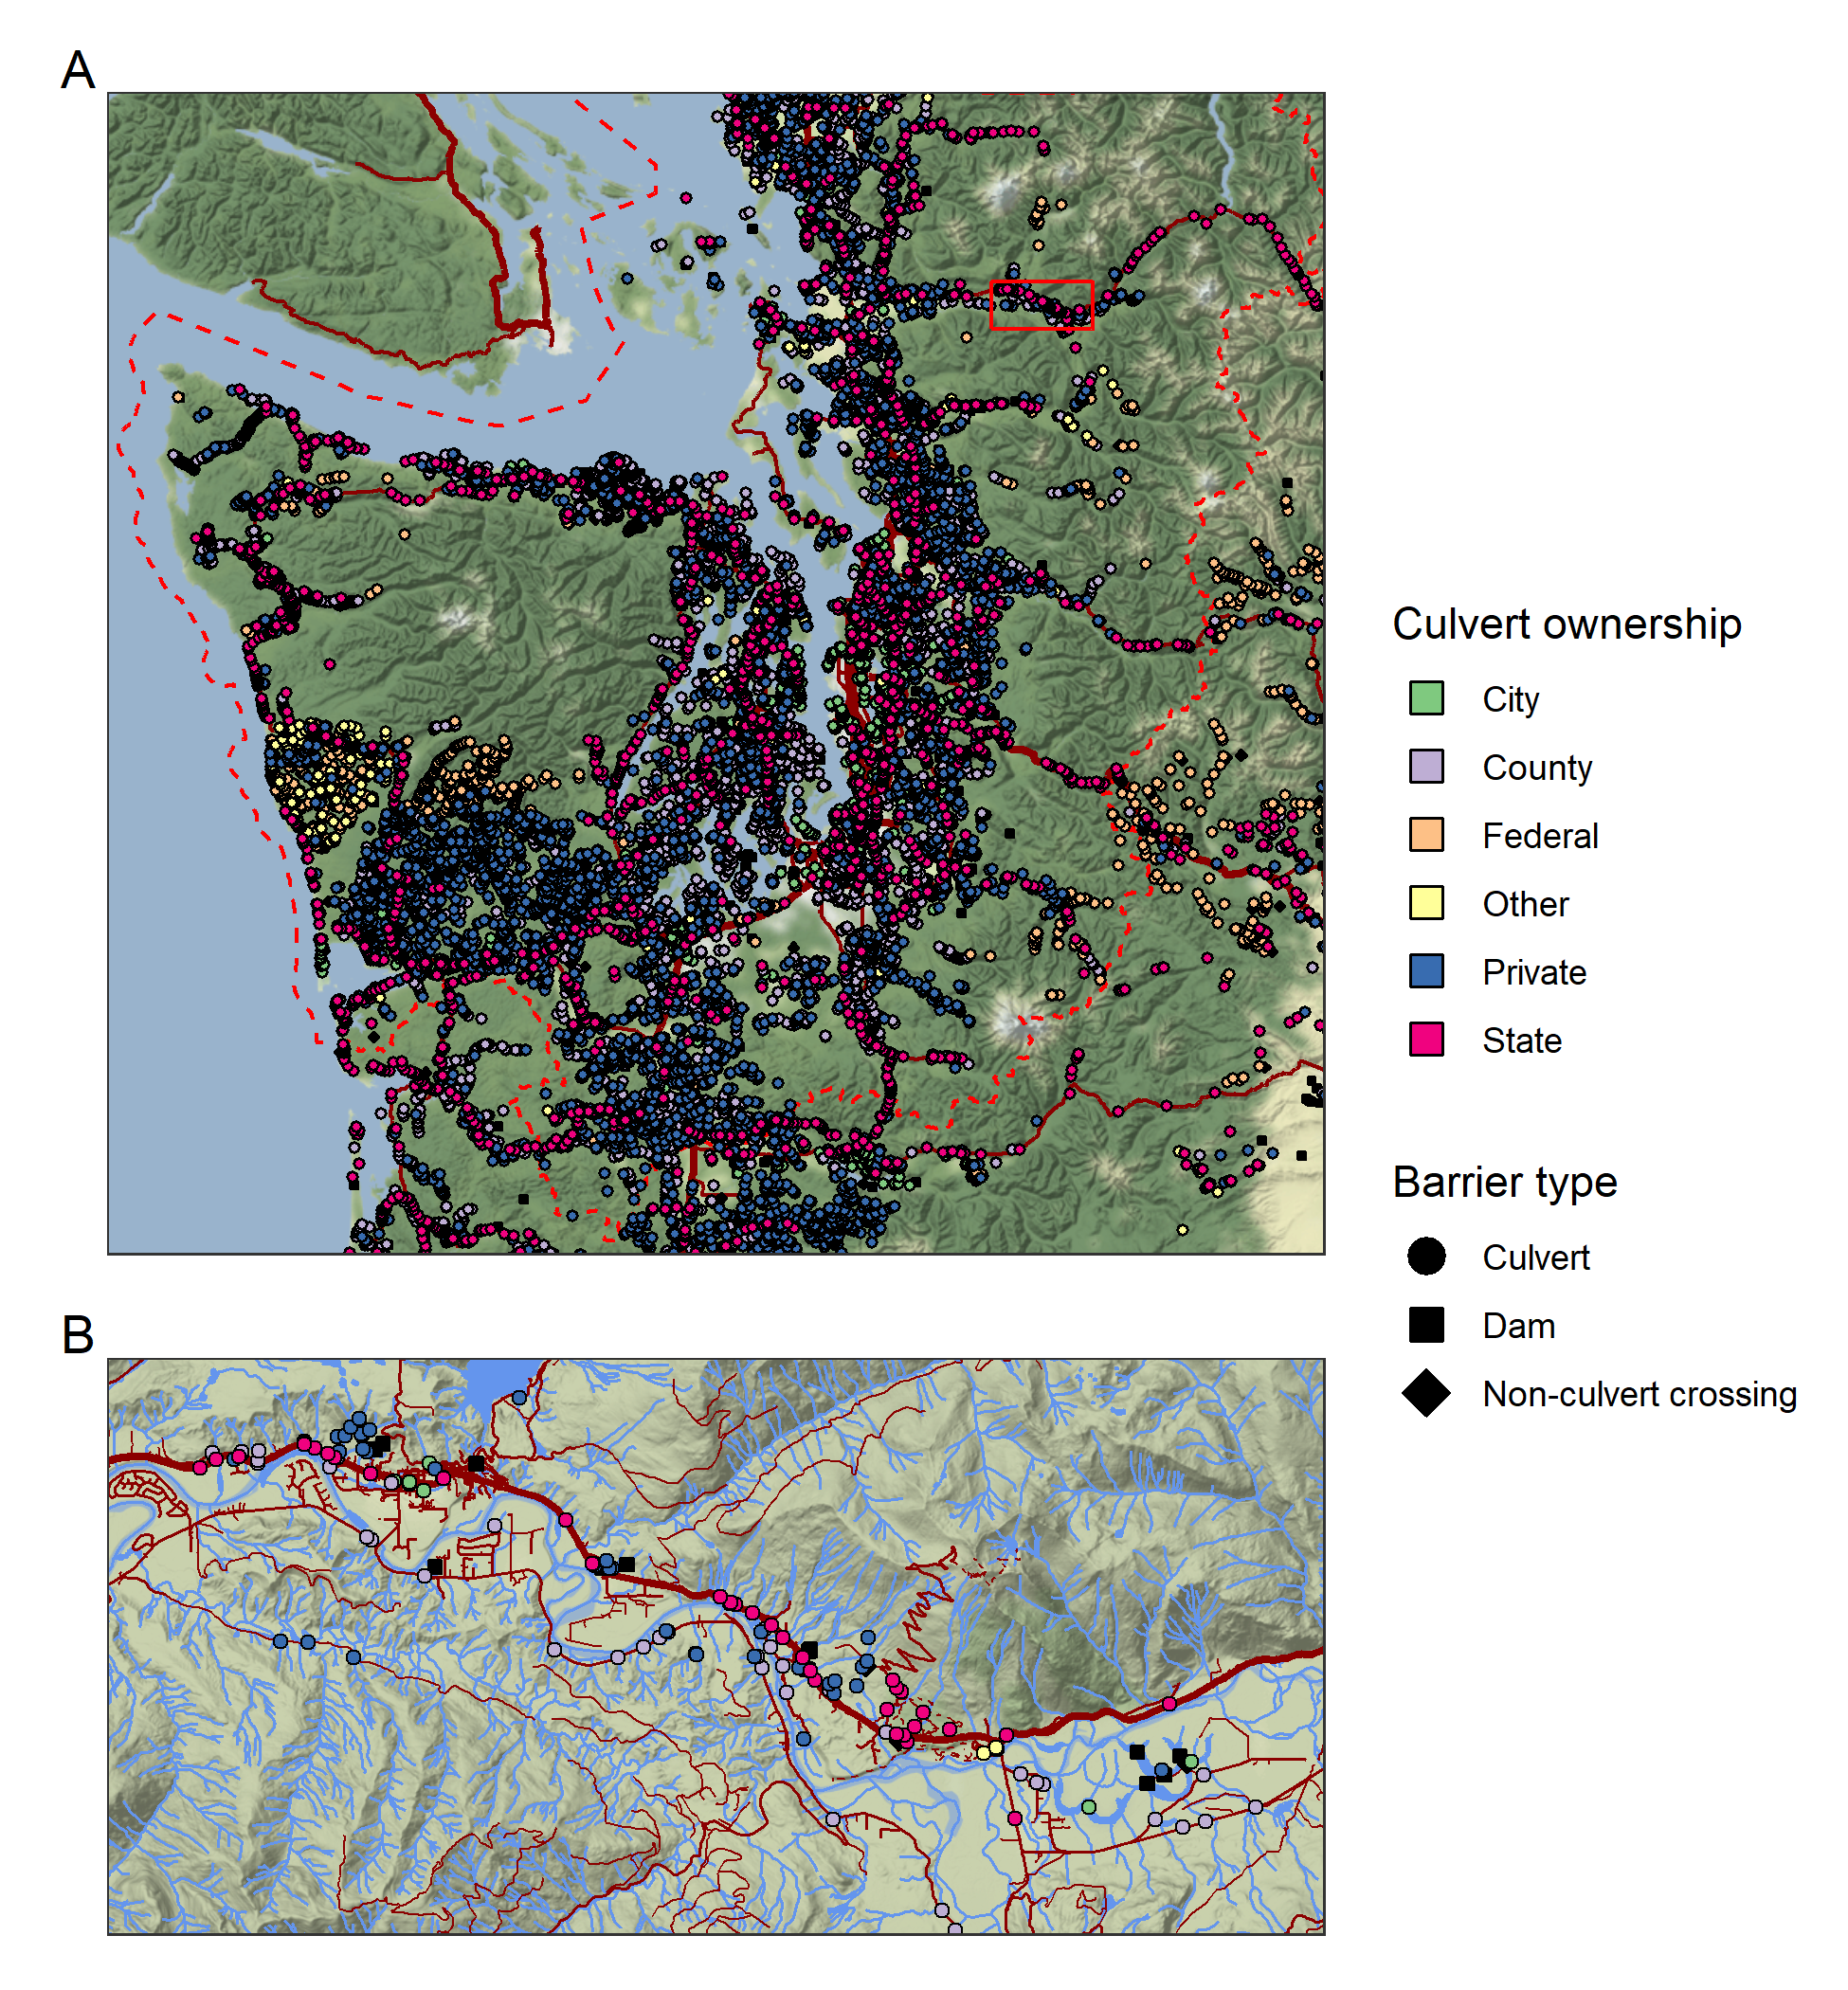
\includegraphics[width=10cm]{figures/fig_mapconcrete.png}
\caption{Barriers to fish passage in the WDFW Fish Passage and Diversion Screening Inventory database by ownership type. (A) shows the entire Case Area (red dotted line) and (B) shows the diversity of barrier ownership entities in the Concrete, WA area along the Skagit River. Solid red box in (A) shows the extent of (B). Dark red lines show roads (data source: OpenStreetMap) and light blue lines show rivers, streams and other water bodies (data source: National Hydrology Dataset High Resolution).\label{fig:barrierMap}}
\end{wrapfigure}%

Migratory anadromous salmon and steelhead native to Western Washington (\textit{Oncorhynchus} spp.) rely on access to diverse stream conditions throughout their spawning and rearing phases of their complex life cycles. Barriers to fish passage, particularly poorly-designed culverts at road crossings, prevent fish from accessing potential habitat, hampering recovery efforts for declining populations \citep{noauthor_2020_2020}. Reconnecting isolated habitat by correcting these culverts has been long identified as a crucial stage in watershed restoration \citep{roni_review_2002}. However, until fairly recently, barrier correction efforts have been limited by lack of available funds and political will. 
%NWIFC State of our Watersheds http://files.nwifc.org/sow/2020/state-of-our-watersheds-sow-2020-final-web.pdf
% Roni, Philip, Timothy J. Beechie, Robert E. Bilby, Frank E. Leonetti, Michael M. Pollock, and George R. Pess. “A Review of Stream Restoration Techniques and a Hierarchical Strategy for Prioritizing Restoration in Pacific Northwest Watersheds.” North American Journal of Fisheries Management 22, no. 1 (2002): 1–20. https://doi.org/10.1577/1548-8675(2002)022<0001:AROSRT>2.0.CO;2.


In 2001, Washington state was sued by the United States Department of Justice on behalf of 21 Northwest tribes for violating treaty fishing rights. The plaintiffs argued that state-owned culverts restrict salmon and steelhead access to historical upstream spawning habitat, leading to declines in salmon abundance and violating the Stevens Treaties which guarantee a right to fish within relinquished tribal lands (referred to as the "Case Area") \citep{hickey_highway_2018}. The lawsuit resulted in a 2013 federal court injunction requiring the state remove barrier culverts under its jurisdiction such that 90\% of blocked fish habitat is made accessible by 2030. The ruling mandates that the remainder of state-owned barrier culverts be restored for fish passage at the end of their life. After nearly two decades of legal battles, in 2018, the U.S. Supreme Court ruled in favor of the tribes, upholding the 2013 federal injunction, ushering in a new era of fish passage policy in Western Washington. 

As of 2020, Washington State Department of Transportation (WSDOT), responsible for the vast majority of state-owned culverts within the Case Area, has corrected 87 injunction barrier culverts opening up an estimated 383.3 miles of habitat at a cost of over \$159 million. Since the ruling, WSDOT has replaced an average of 12.4 culverts per year, including 13 in 2020 \citep{noauthor_wsdot_2020}. To satisfy the federal injunction, the rate of culvert replacements must ramp up dramatically. 
% Cite WSDOT annual report in this paragraph https://wsdot.wa.gov/sites/default/files/2019/09/20/Env-StrRest-FishPassageAnnualReport.pdf

Importantly, the 2013 injunction strictly applies to state-owned culverts whereas there exist an estimated 3,000 and 1,300 additional barrier culverts owned by counties and cities respectively, along with barrier culverts on private lands, often on the same streams as state-owned culverts \citep{brown_coming_2019}. Figure~\ref{fig:barrierMap} shows culvert barriers to fish passage recorded in the Washington Department of Fish and Wildlife (WDFW) Fish Passage and Diversion Screening Inventory (FPDSI) database, (A) for all of the Washington injunction area and (B) along the Skagit River near Concrete, WA as an example of a watershed where barriers owned by several entities exist. Six ownership entity types are indicated, cities, counties, federal, private, state, and other, demonstrating the multiplicity of barrier ownership entities within the region. The presence of multiple barrier ownership entities within a single watershed means that the benefits of any one entity's culvert restoration actions depend on the culvert restoration actions of other actors and suggests potential gains from coordination. While non-state entities are not subject to the 2013 injunction, counties and cities across the region are ramping up their own barrier correction efforts in order to capitalize on the opportunity to restore habitat access throughout the Case Area \citep{brown_coming_2019}. 

However, counties and other actors are largely acting independently and there is heterogeneity between and within these ownership types in terms of goals, priorities, and resources for removing barriers to fish passage. For example, some counties conduct full habitat surveys in determining which barrier culverts to replace first, while others rely on only GIS-based proxies. With regards to funding, while some cities and counties are able to access direct financial resources for fish passage projects, e.g.\ King County has used the surface water management fee to fund culvert restoration projects, other cities and counties do not have access to dedicated funding streams, primarily relying on grant funding.  

Fish passage restoration efforts in Washington state are not entirely uncoordinated. The Brian Abbott Fish Barrier Removal Board was established by the Washington State Legislature in 2014 to recommend priority projects to the Governor's Office and Legislature for funding, thereby promoting the coordinated and strategic removal of barriers to fish passage. In the 2021-2023 biennium, 87 ranked projects were recommended for funding at a total of \$61.3 million. Grant applicants include cities, counties, and non-profit organizations. There is demand from both the Legislature and grantees to better define the Board's selection criteria for potential projects and overall prioritization strategy. 


\subsection{Optimization tools in fish passage}

While there is a rich academic literature applying optimization tools to fish passage \citep{ohanley_optimizing_2005, kuby_multiobjective_2005, mcmanamay_commonalities_2019, couto_safeguarding_2021}, only recently have these tools gained traction with resource managers. Here we highlight two such applications of optimization tools used in fish passage. 

In the fall of 2019 the California Fish Passage Forum announced the launch of a web-based user-friendly optimization DST called \href{https://fishpass.psmfc.org}{FISH\emph{Pass}} to guide strategic planning around fish passage barrier removal across the state \citep{ohanley_optipass_2015}. The development of FISH\emph{Pass} resulted from a collaborative effort between the California Fish Passage Forum, the National Fish Passage Program, the Pacific States Marine Fisheries Commission, and others and is based on the mixed integer linear programming optimization framework developed by \citet{ohanley_optimizing_2005}. The adoption of FISH\emph{Pass} in California replaced rank and score methods with stated goals of improving objectivity in recommendations, providing a systematic framework to project selection given limited financial resources, and balanced multiple and possibly competing objectives and constraints. Currently, the California Fish Passage Forum is funding research that will apply the FISH\emph{Pass} tool to the Smith River watershed to learn about the performance of FISH\emph{Pass} and identify approaches and data inputs to strengthen the model.\footnotemark\footnotetext{See \url{https://www.cafishpassageforum.org/2020-projects} for more detail.} 

A second application is \href{https://greatlakesconnectivity.org}{FishWerks} developed for the Great Lakes region as a collaboration between Cornell University and the University of Wisconsin. The FishWerks DST allows users to generate restoration plans including dam removal and barrier culvert restoration. \citet{moody_pet_2017} identify three necessary features for a DST to bring value to users. First, the underlying data must be dynamic and up-to-date. Second, maintenance must be made easy to ensure use, because organizations rarely have the resources including technical staff to support hosting and maintaining the DST beyond the initial project period. Third, due to a potential perceived black box nature of an optimization DST, the tool must offer significant improvements to the simpler planning methods to ensure adoption. 

Beyond these two applied examples, the fish passage optimization literature includes a multitude of case study applications where the optimization problem or solution methods are tailored to reflect particular ecological or institutional conditions. Our project will identify methods and features from this robust literature necessary to model key elements of barrier correction institutional and ecological conditions in Western Washington and develop new techniques when necessary. For example, while previous work has identified efficiency gains from coordinating barrier correction across watersheds, jurisdictional boundaries, or budget years \textcolor{red}{(Neeson et al. 2015, Milt et al. 2017)} \citep{neeson_enhancing_2015,milt_local-scale_2017}, to the best of our knowledge no previous study of optimal fish passage restoration has explicitly measured efficiency gains from coordinating barrier correction between ownership entities within watersheds or jurisdictional boundaries. 

\subsection{Tailoring optimization for Washington fish passage prioritization}

Our proposed research will develop a data-driven framework for project prioritization, within the injunction area of Washington state, that synthesizes multiple geospatial datasets with statistical economic and ecological models to identify fish passage restoration plans that maximize ecological, social, and economic objectives at a given funding level. Our framework will be used to assess the tradeoffs between key objectives (e.g.\ increasing salmon habitat, an equitable distribution of habitat gains across contingencies, and mitigating investment risk across stocks) as well as gains from coordinating barrier culvert replacement across key actors (e.g.\ the state, counties, and cities) and alternative funding streams. We will make the data, models, and framework accessible to users through an online decision support tool (DST) similar to FISH\emph{Pass} developed for California and Fishwerks developed for the Great Lakes. To our knowledge, our fish passage optimization framework will be the first to include objectives of equity and risk mitigation, allowing resource managers to compare how plans address potentially competing priorities. 

Our framework presents an alternative to the ``rank and score'' methods, or prioritization indices (PI), currently used by Washington State and various other actors (e.g. counties) for prioritizing barrier culverts for restoration. These methods, frequently variations of WDFW's system \citep{noauthor_fish_2019}, are essentially a weighted sum of factors that drive the benefits, and sometimes costs, associated with correcting a single barrier culvert in isolation. Points are assigned based on whether specific metrics, measured via field survey or GIS tools, fall within specified ranges. For example, a PI may be increasing in habitat quantity and quality metrics for all five species of salmon, decreasing in the number of barriers downstream, and decreasing in estimated project cost. 

These indices typically include a significant number of component variables which vary across ownership entities, along resources necessary to consistently generate PI scores. For example, a recently completed inventory of county-owned barriers in Clallam and Jefferson Counties uses a PI that incorporates species-specific intrinsic potential scores for three salmonid species, while another recent report by the City of Bellingham presents a PI that includes bonuses for proximity to WSDOT projects or scheduled roadwork. Distinct PI frameworks across barrier ownership entities prevent consistent comparisons of the relative benefits, or costs, of barrier correction across regions and ownership. 
% WDFW Manual: https://cob.org/wp-content/uploads/2019-fish-barrier-prioritization.pdf

Our proposed DST will build upon existing prioritization frameworks in use across the Case Area in four fundamental ways: 

\begin{enumerate}
\item The scope of our framework includes all barriers in the Washington State injunction area in contrast to barriers under the jurisdiction of a single entity. Including all barriers will facilitate coordination in planning and allow consistent comparisons of the restoration benefits and costs across entities and regions. 
\item We aim to develop planning-level cost estimates for every barrier culvert such that managers can determine which barriers can be restored for a given budget. Our cost estimates are sourced from a statistical model, avoiding the need to obtain costly engineering survey estimates of individual barriers and providing a consistent cost measure across watersheds and ownership entities. 
\item Our tool will explicitly consider stream network structure by assuming there are no habitat gains from upstream barrier culvert correction without first correcting downstream barriers. That is, for a given budget and selection of culverts under the user's control, the tool will suggest a package of culverts to correct or a restoration plan. Any restoration plan identified by the tool will not include an upstream culvert without first including downstream culvert(s), preventing plans that ``strand'' projects by allowing blockages to remain downstream. 
\item Users will have the ability to optimize restoration plans over multiple biological, economic, risk management, and equity objectives using a linear weighting method. A multi-objective framework allows for the explicit examination of tradeoffs between common conservation goals, informing debate about potential alternative paths. 
\end{enumerate}

The utility of our framework and DST critically depends on how well real-world priorities and constraints are reflected. Thus, in the initial phase of the project we will organize a series of workshops where we elicit objectives and constraints from key user groups (see Section~\ref{sec:engage}). For purposes of illustration, here we describe potential factors to be included and the data and models to support their inclusion. As the project progresses, specifics will be adapted to meet stakeholder expectations as discussed during the workshop series.  
%
\section{Approach}
% Some signpost text signalling our overall roadmap.

\subsection{Cost model}

Barrier correction is costly and managers are budget constrained. To incorporate this constraint, we will estimate the cost of culvert restoration for all known existing fish passage-blocking culverts within the US vs.\ Washington injunction area. Culverts in need of restoration will be identified using the FPDSI database maintained by WDFW. Cost estimates will utilize predictive models based on data from over 1,200 culvert projects completed between 2001 and 2015 across Oregon and Washington, documented in the Pacific Northwest Salmonid Habitat Projects (PNSHP) dataset \textcolor{red}{(Katz et al. 2007, NMFS 2020)}. Project records are paired with several predictor variables derived through geospatial matching, including physical features of the worksite (i.e.\ stream slope (\%), bankfull width, road class, elevation, etc.) as well as socioeconomic features (i.e.\ distance to urbanized areas, housing density, proximity to equipment and material suppliers, ownership of nearby land, etc.). In total, over 230 features have been identified as proxies for potential cost drivers and are linked to project records using geospatial matching methods. 

\begin{wrapfigure}{r}{10cm}
	\centering
	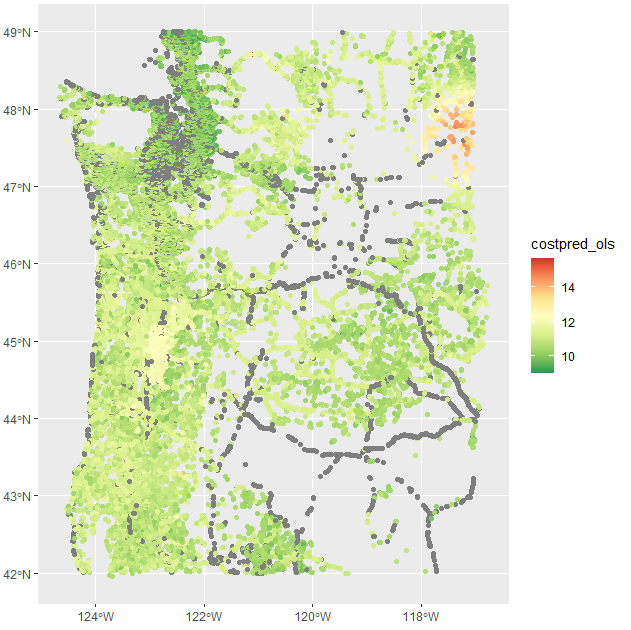
\includegraphics[width=10cm]{figures/predCost.png}
	\caption{Predicted cost percentiles for barrier culverts in the Case Area. Dashed red line indicates Case Area boundary.\label{fig:cost}}
\end{wrapfigure}%

Predictive cost models are currently being finalized by our research team. Figure~\ref{fig:cost} illustrates preliminary predicted cost percentiles using a fit from a boosted regression tree (BRT), one method under consideration. The BRT method builds an ensemble model of iterative regression trees fit on the residuals of earlier fits, systematically identifying variables useful for improving out-of-sample predictive power \citep{elith_working_2008}. In our team's ongoing work, we have found that such models can improve predictive accuracy (measured as training set root-mean square error) by 11\% over predictions from an ordinary least squares fit with variables selected by the analysts. 

For the proposed project, we will leverage the datasets and code we have already developed to explore the predictive performance of several parametric and non-parametric cost models, selecting the model that provides superior out-of-sample predictive power specifically in the injunction area. We will also seek out additional administrative data (i.e.\ project records) from state agencies and large private forestland owners to supplement the PNSHP with additional, region-specific data. In doing so, we will provide consistent and granular barrier correction cost estimates that are applicable over the full Case Area. 

Importantly, our cost estimates will reflect inherent variability in correction costs between barriers. Accounting for heterogeneity in conservation/restoration costs often leads to efficiency gains, as a failure to do so implicitly assumes that all alternatives have the same costs \citep{babcock_targeting_1997,naidoo_integrating_2006}. For example, a recent study found that including cost information in a conservation planning tool increased habitat gains per dollar by as much as an order of magnitude \citep{field_quantifying_2019}. Note that no previous studies in the fish passage optimization literature have used cost estimates based on statistical learning methods such as the BRT predictions demonstrated above. Instead, such studies most frequently rely on heuristic methods that assign barriers to a handful of cost categories (e.g.\ \cite{hermoso_accessible_2021}) or estimates during survey assessments conducted on far fewer barriers (e.g.\ \citep{ohanley_restoring_2013,king_toolkit_2017}), when costs are considered at all. 

\subsection{Habitat model}

A primary objective in culvert barrier correction is increased access to quality salmon habitat. For each culvert restoration plan, defined as a combination of multiple culverts restored, we will quantify the expected increase in habitat quantity, measured as lineal distance, for the five species of Pacific salmon. Spatial dependence will drive restoration benefits, because the culvert restoration downstream determines the benefits from culvert restoration upstream. Estimated habitat quantity gains will be calculated using the USGS National Hydrography Dataset, NDHPlus High Resolution, and the WDFW FPDSI database, which contains information about fish species affected by culvert blockages. Our team has developed code to estimate similar lineal distance metrics for culvert restoration projects in the PNSHP database, which will be leveraged to estimate upstream habitat gained by correcting barriers within the Case Area cataloged in the FPDSI database. 

The lineal distance measures will be supplemented with habitat quality metrics on a per species basis. Prioritization methods currently in use by barrier ownership entities often include some weighting metric for habitat quality. For example, a recent report assessing county-owned culverts in Clallam and Jefferson Counties uses intrinsic potential scores first developed by \cite{burnett_distribution_2007}, while the WDFW methodology assigns a fixed species-specific weight to habitat quantity based on an estimated number of adults potentially produced per habitat area \cite{noauthor_fish_2019}.
% Burnett, Kelly M., et al. "Distribution of salmon‐habitat potential relative to landscape characteristics and implications for conservation." Ecological Applications 17.1 (2007): 66-80.

% Something from Mark?

\subsection{Equity}

Equity is another important dimension to consider. A prioritization framework that simply maximizes expected salmon habitat given a budget constraint could potentially lead to a culvert restoration plan that only benefits a single user group. We will explore alternative equity strategies that prioritize restoration plans that provide an equitable distribution of habitat gains across user groups, e.g.\ watersheds and/or counties. We will also explore various equity metrics, e.g.\ a Gini coefficient, using geospatial data on all salmon runs in the injunction area together with geospatial data delineating watersheds in the Washington State injunction area. 

\subsection{Risk mitigation}

Risk mitigation is yet another important factor to consider when selecting portfolios of barrier culverts to correct. Returns to investments in barrier culvert correction are risky, driven by the possibility of low salmon returns to habitat, population extinction driven by environmental shocks, and future human impacts including impacts to water quality through urbanization \citep{ettinger_prioritizing_2021}. 

Additionally, climate change is expected to be a significant driver of returns to investments from barrier culvert correction. Climate change is projected to affect peak water flow during egg incubation, stream temperature during pre-spawning, and minimum flow during spawning \citep{battin_projected_2007}, with greatest impacts in high-elevation streams where barrier culverts are less common. Climate change may also affect channel bankfull width at road crossings, which in turn may cause a previously corrected culvert to revert to barrier status as the stream expands under future climate conditions. While expanded culvert designs can prevent this, they are often more expensive \cite{guillaume_mauger_climate_nodate}. Climate uncertainty will thus create risk of future culvert failure when smaller, cheaper correction designs are considered. 
% Mauger,  G.S., S.Y.  Lee, J.S.  Won, K.  Byun, and  A.F. Hamlet, 2018. Climate  robust culvert design: Probabilistic estimates of fish passage impediments. Final report for the Skagit Climate Science Consortium. Climate Impacts Group, University of Washington, Seattle. https://cig.uw.edu/wp-content/uploads/sites/2/2018/07/Final_Report_SC2-Culverts_FINAL.compressed_3.pdf

Drawing from the literature on restoration portfolio diversification, we will estimate the degree to which the risk in returns to barrier culvert removal plans can be mitigated through diversification. We will explore risk metrics ranging in complexity from a simple measure of the spread of investments across all salmon runs with habitat in the injunction area to increasingly complex risk metrics that utilize information on the potential negative covariance in expected returns to multiple salmon populations to exploit opportunities for portfolio diversification \citep{sanchirico_empirical_2008, jardine_fishermen_2015, johnston_combining_2002}.  

%\subsection{Network configuration}
%\subsection{Ownership}
\clearpage
\subsection{Optimization Framework\label{sec:opt}}

\subsubsection{Design}
\begin{wrapfigure}{r}{0.5\textwidth}
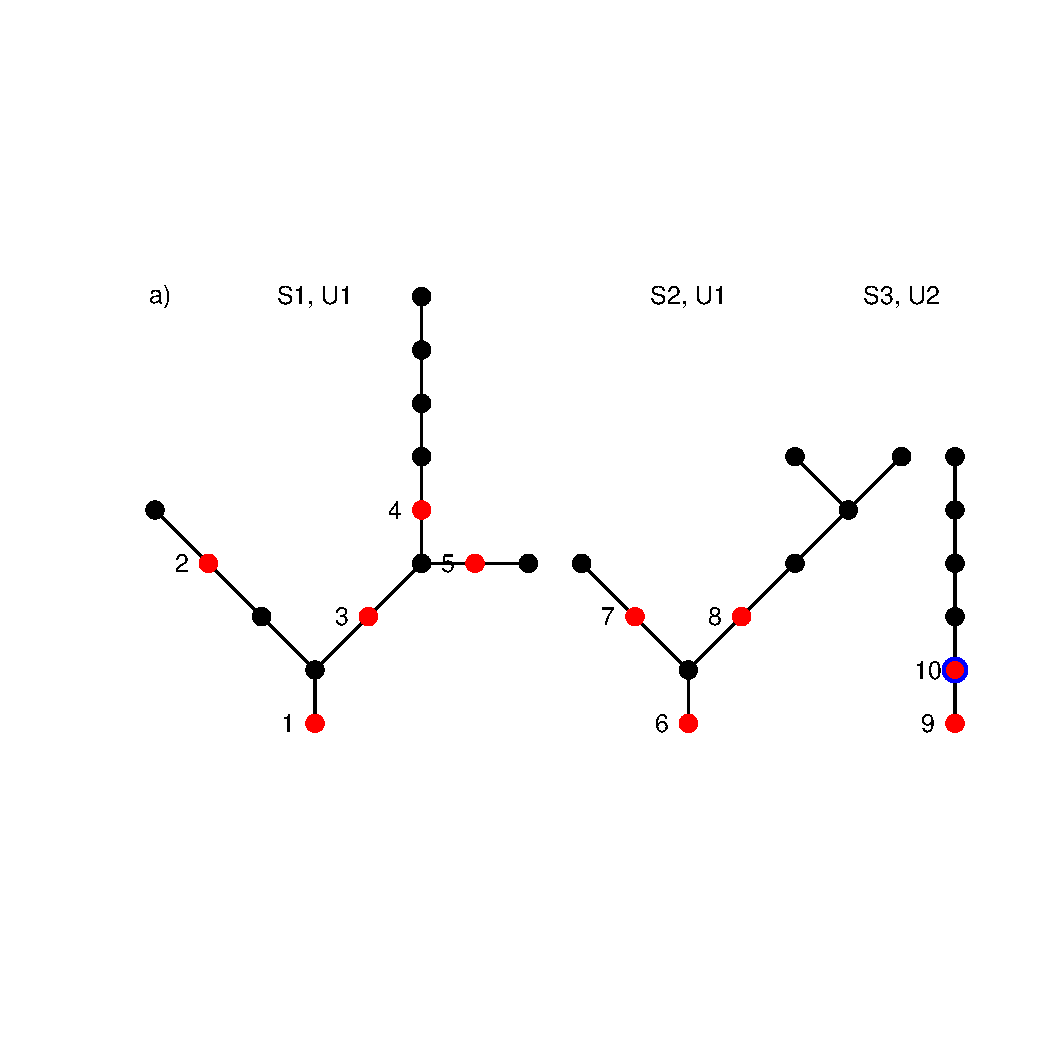
\includegraphics[width=0.48\textwidth]{figures/opt_s.pdf}
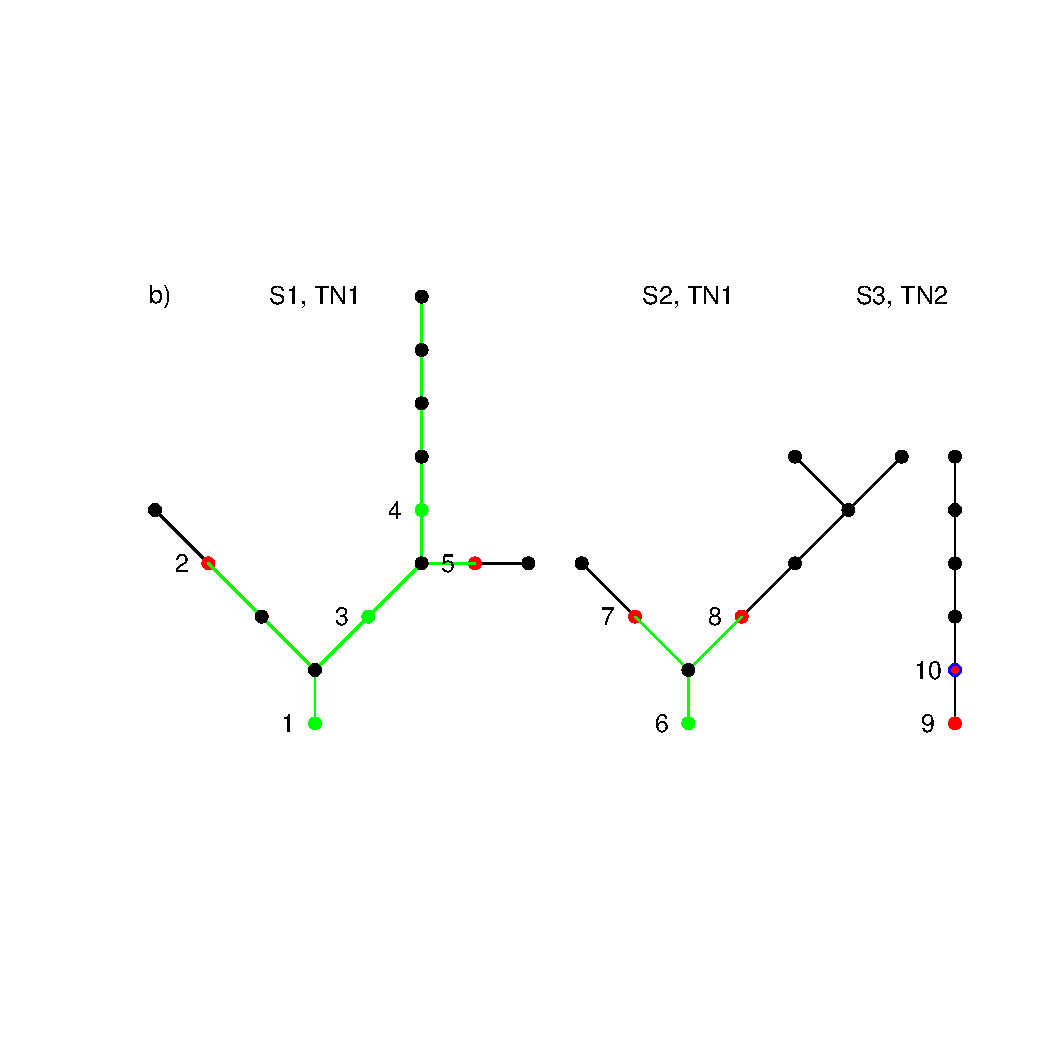
\includegraphics[width=0.48\textwidth]{figures/opt_h.pdf}
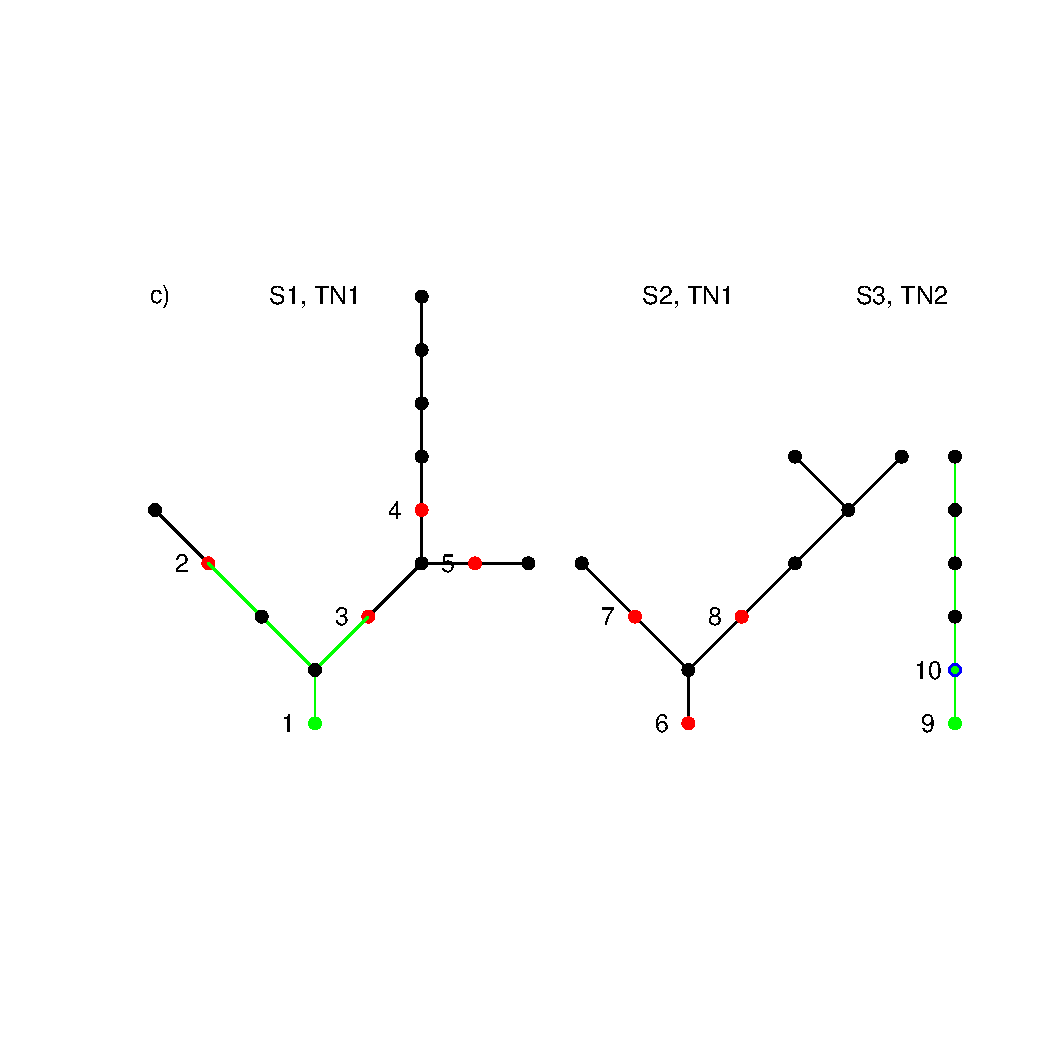
\includegraphics[width=0.48\textwidth]{figures/opt_e.pdf}
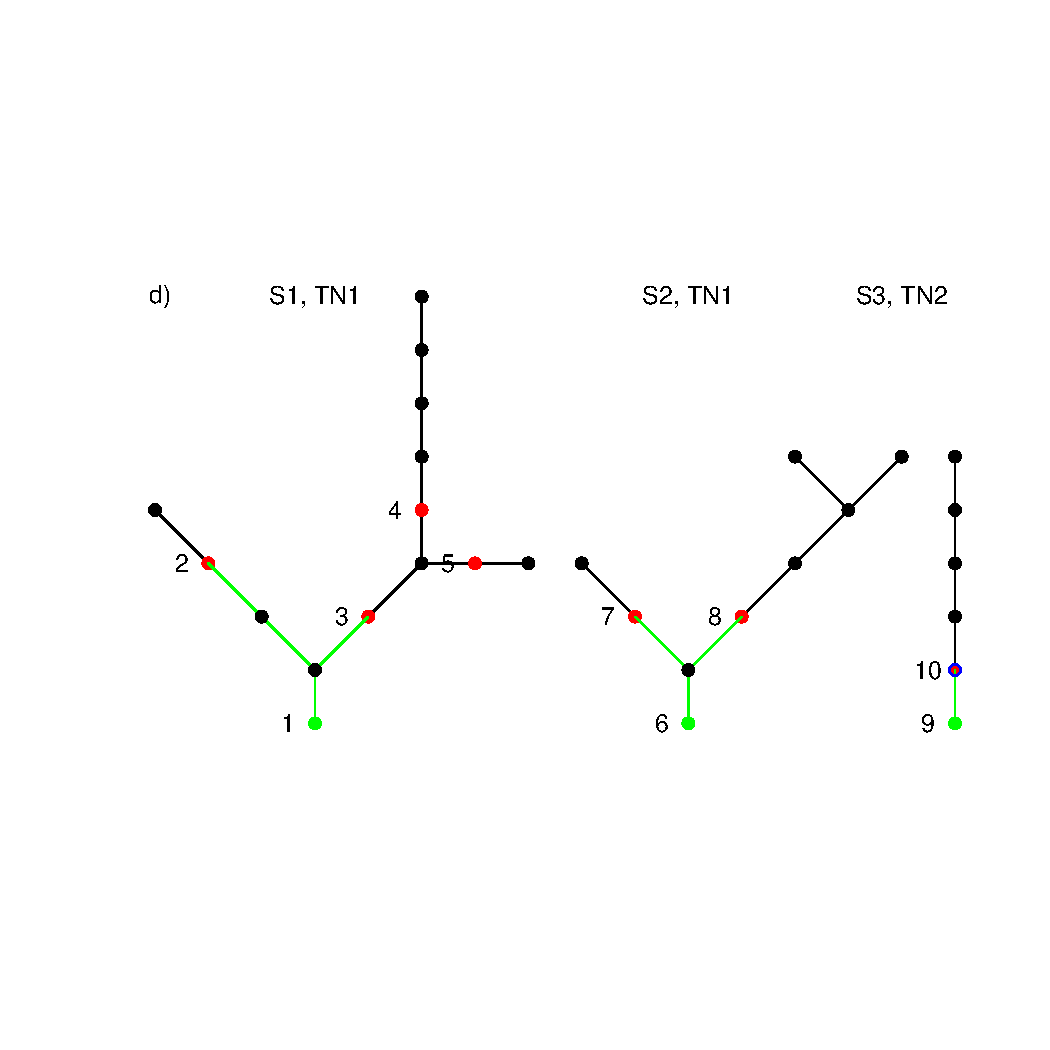
\includegraphics[width=0.48\textwidth]{figures/opt_d.pdf} 
\caption{Solutions to a scalarized multiobjective problem in a stylized system where there are three salmon stocks (S1-S3) and two tribal nations (U1-U2). \label{fig:opt}}
\end{wrapfigure}%


We will explore two alternative approaches to define cost-effective restoration plans that meet multiple planning goals (e.g.\ salmon habitat gains, equity considerations, and risk mitigation). Both approaches are considered ``a priori'' methods for multiobjective optimization because the decision maker must specify their preferences related to the various objectives prior to the optimization. 

In the first approach (i.e.\ linear scalarization), managers specify importance weights for each of the objectives and the weighted sum of the objectives is maximized. Weights are constrained to the interval [0, 1] and sum to one, e.g.\ a manager solely interested in habitat would set the habitat importance weight to one and all other weights to zero. The problem will also include a budget constraint, such that expenditures on barrier restoration are less than or equal to a fixed budget $B$, and a hydrography constraint such that habitat gains from restoring any one barrier cannot be realized if there exist any downstream barriers to fish passage. Figure~\ref{fig:opt} demonstrates solutions to this first optimization approach with a budget constraint of \$40. Panel (a) represents a model system with 10 barrier culverts (numbered red markers), 26 units of potential habitat (increments between two adjacent markers represent one unit of habitat), on three streams utilized by three salmon stocks (S1-S3), harvested by two user groups (U1-U2). Each of the culverts 1-9 have correction cost \$10 to restore while culvert 10 has correction cost \$20 (outlined in blue).

Panel (b) represents the habitat-maximizing solution (the habitat weight is set to one and all other weights are set to zero), with 14 units of habitat gained (11 on stream 1 and three on stream 2), but all of the benefits going to a single user group. In the habitat-maximizing solution, the budget is exhausted by restoring four culverts for a total cost of \$40. Panel (c) represents the equity-maximizing approach (the equity weight is set to one and all other weights are set to zero), with nine units of habitat restored (four on stream 1 and five on stream 3). In this solution, the budget is also exhausted and the habitat gains are nearly evenly split across tribal nations (four for U1 and five for U2). Finally, panel (d) represents the diversification-maximizing solution (the weight on diversifying habitat gains across salmon stocks is set to one and all other weights are set to zero), with a total of eight units of habitat gained (four on stream 1, three on stream 2, and one on stream 3) spread across the three salmon stocks. Interestingly, the budget is not exhausted in the diversification-maximizing solution as total expenditures for the three culverts restored is \$30. Whenever objective functions are defined by even allocations, e.g.\ across user groups or salmon stocks, the budget constraint may not hold. 

In the second approach (i.e.\ $\epsilon-$constraint method), one objective function is maximized and lower bounds, $\epsilon$ parameters are provided for all remaining objectives. For example, the problem can be defined to maximize habitat gains subject to each user group receiving some minimum fraction of the habitat gains or some minimum fraction of total expenditures, or a constraint such that habitat gains are distributed across some minimum number of salmon stocks. 

The problem will be solved using R, a free software environment that supports integer programming. The user interface to the prioritization framework, or DST, will be an online app created with the Shiny package for R and hosted on the Shiny Server. Similar tools have been built using various proprietary software programs \citep{ohanley_optipass_2015, moody_pet_2017, mcmanamay_commonalities_2019}. Through using an open-source optimization framework coupled with an open-source user interface we maximize accessibility and customizability. 

\subsubsection{Applications}
% More about the DST here?

Under the mentorship and supervision of PI Jardine and mentorship of co-PI VanDeynze the Sea Grant Fellow will utilize our framework to explore the following research questions as the basis of a masters or PhD thesis: 

\begin{enumerate}
%\item How can equity be accounted for in in fish passage problems? (Note, to our knowledge equity has not been accounted for in the fish passage prioritization literature.)
%\item How can project risk be accounted for in fish passage problems? (Note, to our knowledge risk has not been accounted for in the fish passage prioritization literature.)
\item What are the gains in benefits, e.g.\ habitat, equity, and risk avoidance, associated with coordination across actors (state agencies, local government, private landowners) and which of these multiple objectives is most affected by a lack of coordination across actors? 
\item Where in Washington injunction area (sub-basins/watersheds) are culvert restoration plans associated with trade-offs between potentially competing priorities (e.g., risk versus total habitat, equity versus total habitat), and where can "win-wins" occur (i.e., plans that meet multiple objectives without reducing others)? 
\item How do the two optimization approaches, i.e.\ linear scalarization and the $\epsilon-$constraint method, compare in terms of solution stability and computational efficiency, and which of the two approaches is preferred by stakeholders in terms of ease of use and interpretability. 
\end{enumerate}


\subsection{Role of team members and partners}
\textbf{PI Jardine} will serve as the lead administrator of the grant where administrative responsibilities include organizing meetings both internally and with the scientific advisory board to ensure the project is on track to deliver work products on time, tracking project performance, facilitating project design decisions, and supervising and mentoring the postdoctoral scholar, the Sea Grant Fellow, and the SMEA Research Assistant.  PI Jardine will also provide technical assistance with optimization in R and developing the R Shiny app including providing template code for various optimization algorithms along with sensitivity analyses and model selection, and providing template code for the DST user app features.\\


\textbf{Co-PI Van Deynze} will co-administer the grant, with PI Jardine, where administrative responsibilities include organizing meetings both internally and with the scientific advisory board to ensure the project is on track to deliver work products on time, tracking project performance, facilitating project design decisions, and mentoring the Sea Grant Fellow and the SMEA Research Assistant. Co-PI Van Deynze will also assist with developing and deploying the optimization algorithm and the R Shiny app. As a post-doctoral research associate, co-PI Van Deynze will receive training from PI Jardine in the development of applied optimization algorithms, in project administration, and in mentorship of students, furthering development as an independent researcher. \\

\textbf{Co-PI Fonner} will provide assistance as needed for development and deployment of the multi criteria optimization framework and corresponding algorithm. He will also support the engagement and outreach effort, facilitating incorporation of best practices and paradigms from conservation social sciences. Additionally, co-PI Fonner will provide guidance on the institutional environment and human dimensions associated with salmon conservation and recovery.\\

\textbf{Co-PI Scheuerell} will ....\\

\textbf{Co-PI Holland} will ....\\

The \textbf{SMEA Research Assistant} will catalog methods and datasets for fish passage prioritization indices for all counties, and any other entities using prioritization indices, within the Case Area. The RA will also determine the data availability of variables used in the prioritization index of each entity for all barrier culverts in the Washington State injunction area. Through their work, the RA will become deeply familiar with a diverse set of prioritization methods and the practical considerations of their design (e.g.\ resource, information, and interpretability constraints), preparing them for a professional role in resource policy or further graduate studies. \\

The \textbf{Sea Grant Fellow} will utilize the optimization framework to explore gains from coordinating barrier culvert restoration efforts in Washington State, the trade-offs between various dimensions in the objective function (e.g. the trade-off between total habitat gained and mitigating investment risks in particular stocks), and the practical side of designing complex DSTs that are easy to use and understand for broad audiences. Under the supervision of PI Jardine, the Sea Grant Fellow will compose a student thesis reporting the results of these analyses, providing training in scientific writing. \\

Our team will engage with community partners, including municipal, state, and tribal resource managers and user groups, throughout the term of the project. Our community partners will provide data for informing sub-models and feedback on the optimization framework and DST (see Section~\ref{sec:engage}).

\subsection{Potential challenges}

%
\section{Engagement plan \label{sec:engage}}

\subsection{Community collaborators} 

Our project will by guided by a Fish Passage Policy Advisory Committee (FPPAC) (Table~\ref{tab:sab}) comprised of community collaborators. At each phase of our engagement plan, outlined below, we will rely on advice from our Advisory Committee. Members of FPPAC will include individuals working directly in the area of barrier culvert restoration, individuals with a history of engaging with our key stakeholder groups, and individuals generating science relevant to our problem area. The FPPAC already has committed representation from the Squaxin Island Tribe, the Tulalip Tribes, Washington State Recreation and Conservation Office, King County Fish Passage Restoration Program, and Washington Sea Grant. At the time of the submission of this proposal, we are actively seeking to expand this group to representation from other barrier ownership entities and stakeholders. 

\begin{table}[h]
\caption{Fish Passage Policy Advisory Committee (FPPAC) \label{tab:sab}}
\centering
\begin{tabular}{lcc}\hline
 Name & Job Title & Affiliation  \\\hline
Jeff Dickison& Asstistant Natural Resources Director &  Squaxin Island Tribe\\
& & Natural Resource Center\\
\rowcolor[gray]{.9} Steve R Hinton &  Conservation Scientist&  Tulalip Tribes  \\
\rowcolor[gray]{.9}& &Treaty Rights \& Government Affairs\\
Marc Duboiski & Outdoor Grants Manager & Washington State Recreation\\
& & and Conservation Office\\
\rowcolor[gray]{.9}Dave Caudill & Outdoor Grants Manager & Washington State Recreation\\
\rowcolor[gray]{.9}& & and Conservation Office\\
Evan Lewis &  Fish Passage Projects Manager&  King County  \\
& & Fish Passage Restoration Program\\
\rowcolor[gray]{.9}Melissa Schutten & Equity, Access \& Community  & Washington Sea Grant \\
\rowcolor[gray]{.9}& Engagement Lead & \\
\hline
\end{tabular}
\end{table}


\subsection{Target audiences}

There are three main target audiences for our work. First, stakeholders who are directly invested in the outcomes from barrier culvert restoration in Washington state, but are not actively funding barrier culvert restoration projects. Our second target audience includes managers making decisions over which barrier culverts to replace in a given time period with a fixed budget. These managers may be interested in crafting restoration plans for only a subset of barrier culverts in Washington, e.g.\ barrier culverts under the jurisdiction of a particular county, or they may be interested in identifying restoration plans that maximize returns on investment regardless of ownership, e.g.\ members of the Brian Abbott Fish Barrier Removal Board. We view our first and second target audiences as potential users of our DST where the purpose of use is to inform barrier culvert restoration in the Washington State injunction area. Thus, we intend to design the tool to reflect their priorities, objectives, and design the framework and tool to be intuitive to this target audience in terms of use and interpreting the results.

Our third target audience is the general public, including academics, who are interested in lessons learned from natural resource management problems. We view individuals from our third target audience as potential users of our DST in the sense that the DST may be adapted for other problems (areas, species) or expanded on to include other dimensions. The features of the public-facing DST will serve an educational purpose, demonstrating the complexities of managing riparian systems in a concrete setting. 

\subsection{Engagement activities}

In the beginning of YR1, in the initial phase of the project, we will organize a series of workshops intended to uncover the objectives and challenges in culvert barrier replacement for key user groups including WSDOT, city and county governments, restoration funding agencies such as the Fish Barrier Removal Board, WDFW, and representatives from relevant tribal nations. The workshops will begin with a presentation of our proposed framework and online tool as a straw-man proposal in order to generate discussion and elicit ideas on how to capture fundamental real-world priorities and constraints in barrier culvert removal. We will gather feedback during the workshops and through post-workshop surveys. Ideas coming from the initial series of workshops will be incorporated into our project to the extent possible given data and computational limitations, which will be made clear to workshop participants.

In a second phase, at the beginning of YR2, we will organize a second series of workshops to present preliminary results (e.g.\ tradeoffs between various objectives) and demonstrate the functionality of two preliminary working versions of the online tool. One version of the tool will be based on the linear scalarization approach to optimization and the other will be based on the constraint-based method (see Section \label{sec:opt}). This second series of workshops will demonstrate how feedback from the initial workshops was incorporated in our framework and tool and provide a more in-depth discussion of our data inputs to the tool, e.g.\ a demonstration of the quality of our cost estimates and a visual demonstration of our preliminary spatial definition of our equity metric. The second series of workshops will provide stakeholders with a final opportunity to guide key features of the framework and solicit feedback on the usability of the online DST and the optimization approach perceived to be most intuitive. 

Finally, at the end of YR2, we will host an interactive workshop to launch our finalized online tool letting stakeholders directly engage with the tool. In preparation for this workshop, we will develop a video tutorial that will present content from the DST user guide in a way that is accessible and engaging. The workshop will begin with a screening of the video tutorial. Then, we will engage participants with exercises that highlight the tradeoffs between various objectives, gains from coordination, and how alternative budget/funding scenarios (defined by budget levels and their distribution across time) impact the culvert restoration packages with the highest return on investment. Each workshop participant will be provided with a laptop computer to participate in the exercises. 

\subsection{Anticipated outcomes and evaluation}

%We anticipate two major research outcomes. First, our research will form the basis of a student thesis, leading to a scientific publication, applying our underlying optimization model to answer important research questions including:
%
%\begin{enumerate}
%\item How can equity be accounted for in in fish passage problems? (Note, to our knowledge equity has not been accounted for in the fish passage prioritization literature.)
%\item How can project risk be accounted for in fish passage problems? (Note, to our knowledge risk has not been accounted for in the fish passage prioritization literature.)
%\item What are the gains in habitat, equity, and risk avoidance associated with coordination across actors (state agencies, local government, private landowners) and which of these multiple objectives is most affected by a lack of coordination across actors?
%\item Where in Washington injunction area (sub-basins/watersheds) are culvert restoration plans associated with tradeoffs between potentially competing priorities (e.g., risk versus total habitat, equity versus total habitat), and where can "win-wins" occur (i.e., plans that meet multiple objectives without reducing others)?
%\item How do the two optimization approaches, described in Section~\ref{sec:opt}, compare in terms of how solution stability, computational efficiency, and which of the two approaches is preferred by stakeholders.
%\end{enumerate}
%
%
%Second, our project will produce publicly-available, well-documented, open-source prioritization DST for barrier culvert removal in the Washington injunction area. The DST can serve a coordinating function by providing a framework to evaluate restoration plans across various actors regardless of whether the restoration plan is one identified by our optimization framework. The DST can also support planning for cities and counties with limited access to data and quality cost estimates. Finally, the source code behind our open-source DST will be made widely available to users outside of the state of Washington to facilitate the adoption of and customization by a larger set of potential users. 

\subsection{Estimated costs}

\clearpage
\large References\\
\normalsize
\bibliography{wsg-bvd}
\end{document}